\documentclass[a4paper]{article}

% Для того чтобы задать нестандартный 14-ый размер шрифта
\usepackage[14pt]{extsizes} 

% Поддержка русского языка
\usepackage[utf8]{inputenc}
\usepackage[russian]{babel}
\usepackage{setspace,amsmath}

% Настройки полей документа
\usepackage[left=20mm, top=15mm, right=15mm, bottom=15mm, nohead, footskip=10mm]{geometry} 

% Нормализация первого абзаца
\usepackage{indentfirst}

% Нумерация секций выкл.
\pagestyle{empty} 

% Межстрочный интервал
% \linespread{1.3}

\usepackage{textcomp}
\usepackage{ tipa }

%Графики
\usepackage{graphicx}
\graphicspath{{pictures/}}
\DeclareGraphicsExtensions{.pdf,.png,.jpg}

\begin{document}
	
	\section*{Спектральное регулирование запаса реактивности путем изменения состава теплоносителя (H$_2$O + D$_2$O)}
	
	\subsection*{Зависимость коэффициента размножения от процентного содержания D$_2$O в смеси}
	
	С помощью программы GETERA была найдена зависимость K$_{\infty}$ от процентного содержания D$_2$O в смеси ($\delta_{\text{D}_{2}\text{O}}$), которая представлена на рисунке \ref{ris:deltaOtK}.
	
	\begin{figure}[h]
		\centering{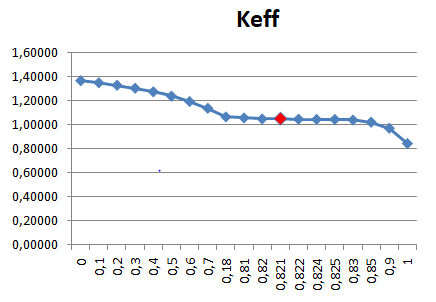
\includegraphics{deltaOtK}}
		\caption{Зависимость K$_{\infty}$ от $\delta_{\text{D}_{2}\text{O}}$}
		\label{ris:deltaOtK}
	\end{figure}

	Далее был выполнен расчет жесткости спектра нейтронов при различных значениях $\delta_{\text{D}_{2}\text{O}}$. Изменение спектра нейтронов в зависимости от разбавления, показано на рисунке \ref{ris:spectr}.
	
	\begin{figure}[h]
		\centering{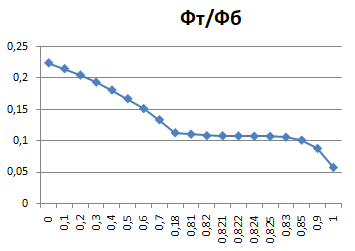
\includegraphics{spectr}}
		\caption{Зависимость Ф$_\text{Т}$ / Ф$_\text{Б}$ от $\delta_{\text{D}_{2}\text{O}}$}
		\label{ris:spectr}
	\end{figure}
	
	Также было найдено значение $\delta_{\text{D}_{2}\text{O}}$, при котором K$^{Begin}$$_{\infty}$ = 1.05 для разных обогащений по $U_{235}$. Далее был произведен расчет выгорания при однократной перегрузке для двух случаев: при осуществелении спектрального регулирования путем изменения процентного содержания D$_2$O в смеси и в случае, когда замедлитель просто обычная вода. 
	Все значения представлены в таблице \ref{table:vygoranie1}.
	
	\begin{table}[h]
		\caption{Значения выгораний и выйгрыш для разных обогощений по $U_{235}$}
		\label{table:vygoranie1}
		\begin{center}
			\begin{tabular}{|c |p{100pt} | p{100pt} | c | c |}
				\hline
				x, \% & Выгорание  D$_2$O, MBт/сут &Выгорание  Н$_2$O, MBт/сут & $\delta_{\text{D}_{2}\text{O}}$, \%  & выйгрыш, \% \\ 
				\hline
				$4,95$ &  $41,9$ & $36,2$ & $85$ & $13$ \\
				\hline
				$5,5$ &  $47,6$ & $42,4$ & $87,5$  & $11$ \\
				\hline
				$6,0$ &  $52,8$ & $48,3$ & $89$ & $9$ \\
				\hline
				$6,5$ &  $56,1$ & $51,3$ & $91$ & $8$ \\
				\hline				
			\end{tabular}
		\end{center}
	\end{table}

	Из результатов видно, что повышение обогащения нецелесообразно так, как не увеличивает выйгрыш в выгорании, а, наоборот, уменьшает его.
	
	Далее, было посчитано накопление плутония и построены графики зависимости концентрации плутония, от времени с начала работы. Сначала был рассмотрен вариант однократной перегрузки со спектральным регулрованием и без(рисунок \ref{ris:pu1}). Видно, что при спектральном регулировании накапливается больше плутония, который должен включиться в работу и повысить выгорание.
	
	\begin{figure}[h]
		\centering{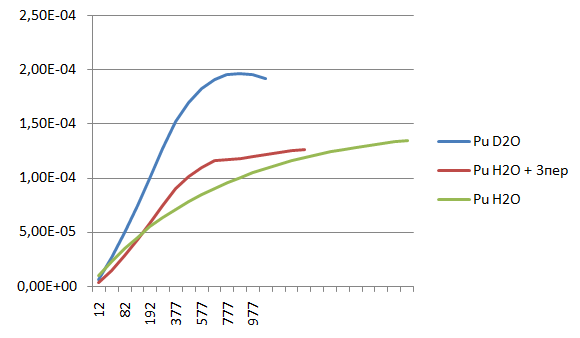
\includegraphics{pu1}}
		\caption{Зависимость концентрации плутония от времни с начала работы со спектральным регулированием и без}
		\label{ris:pu1}
	\end{figure}
	
	Потом было рассмотрено накопление плутония для различных обогащений по урану 235 со спектральным регулированием.
	\begin{figure}[h]
		\centering{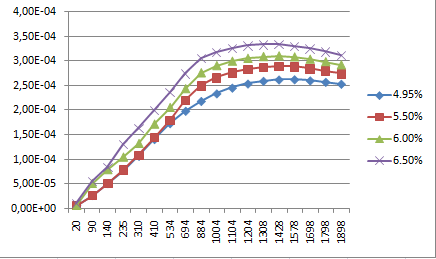
\includegraphics{pu2}}
		\caption{Зависимость концентрации плутония от времни с начала работы со спектральным регулированием при различных обогащениях по $U_{235}$}
		\label{ris:pu2}
	\end{figure} 
	
	Далее были произведены двойные перегрузки со спектральным регулированием и без. Выигрыш в выгорании при спектральном регулировании составил 11\%, а накопление плутония показано на рисунке \ref{ris:pu2n}. Из графика видно, что при спектральном регулировании накапливается больше плутония.
	
	\begin{figure}[h]
		\centering{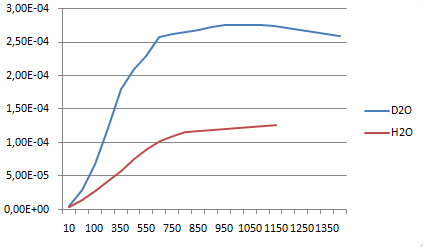
\includegraphics{pu2n}}
		\caption{Зависимость концентрации плутония от времни с начала работы со спектральным регулированием и без при двойных перегрузках, x = 4,95\%}
		\label{ris:pu2n}
	\end{figure} 
	
	
\end{document}
	